\section{Introduction} % (fold)
\label{sec:introduction}
    % Set up introduction.
    The aim of the project was to construct a viable 3D visual representation of the University of Queensland's St Lucia campus.
    The rationale for undertaking this project was multifaceted; it is a thematic continuation of the previous data visualisation project, and it serves as a useful and relevant application of computer graphics techniques.\\

    % What:
    Following the initial proposal, the end goal of the project was to create a visually recognisable recreation of the UQ St Lucia campus.
    In order to accomplish this, multiple computer graphics techniques were utilised to produce the end result.\\

    % Why:
    The previous data visualisation project aimed to analyse the relationships between the faculties, courses, majors, and programs offered by UQ.
    This project is a continuation of the UQ centric theme, however not much else is continued through into this project.

    The rationale of visualising the St Lucia campus in a three dimensional model is to provide a better method of gaining a spatial awareness of the campus' layout and structures.
    This stems from recalling the unhelpfulness of most UQ maps when trying to navigate the campus for the first time.
    Due to the odd shapes of many buildings, the presence of many annexes and similarly labelled and named buildings, the ambiguity between roads, walkways, and viable pathways, and the dense arrangement of buildings, sufficiently learning the layout of the campus may even take weeks.

    \begin{figure}[H]
        \centering
        \fbox{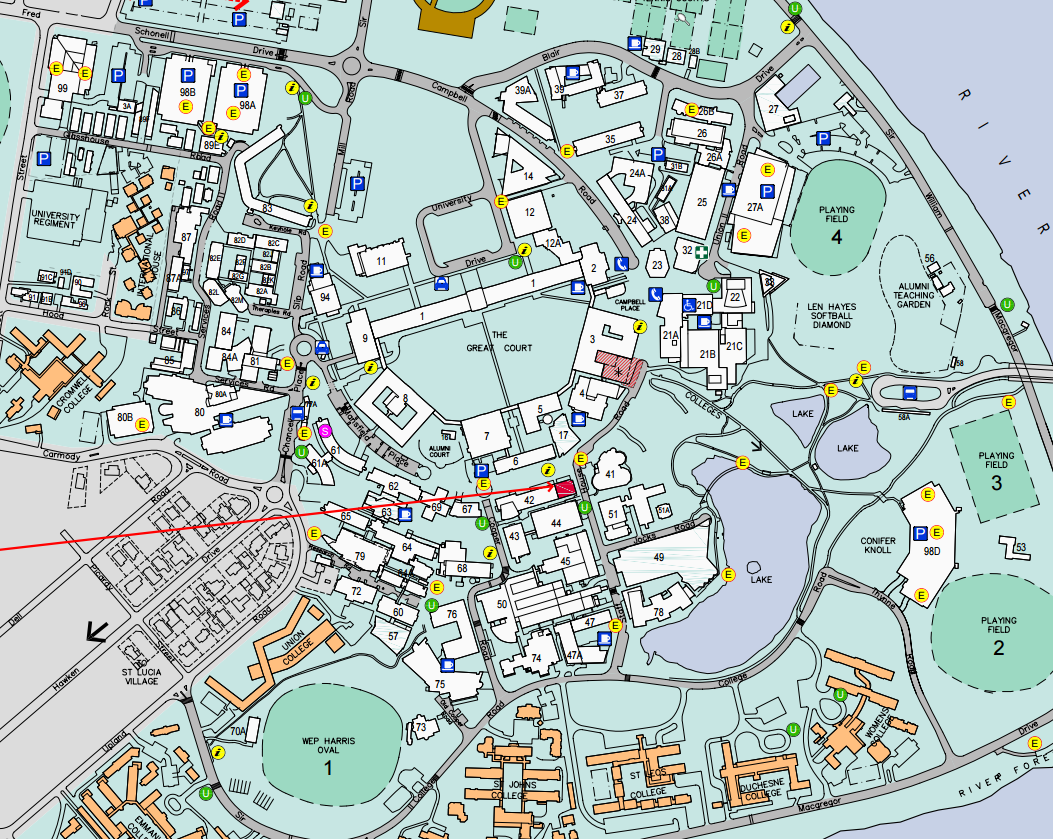
\includegraphics[width=0.75\textwidth]{map}}
        \caption{
            Official University of Queensland St Lucia map \cite{uq_map}. Note the densely packed, oddly shaped and often conjoined layout of the buildings.
        }
        \label{fig:uq_flat_map}
    \end{figure}

    Static maps, such as in Figure \ref{fig:uq_flat_map}, can have high technical accuracy, but are often convoluted and typically don't convey a good physical model of an environment to a reader.
    Abstract two dimensional maps typically require a lot of cross checking between the map and the physical surroundings, in order to correlate real landmarks with what the map displays.
    If structures and landmarks could be better represented to correlate with their real life counterparts more realistically, users will be able to visualise and integrate a locale much more quickly and effectively than attempting to correlate an abstract diagram to their surroundings.


% section introduction (end)
